%-----------------------------------------------------------------------------
%  farelo_choupo.tex -- a ~30 min IST/DEQ department talk.
%  The philosophy and architecture of Choupo (open, glass-box process simulator),
%  its electrolyte model and numerical method, and how the solubility data of
%  Prof. Fatima Farelo enters, validates and recalibrates it.
%  Build:  pdflatex farelo_choupo.tex   (twice).  Figures: figs/*.pdf
%-----------------------------------------------------------------------------
\documentclass[aspectratio=169,11pt]{beamer}
\usetheme{Madrid}
\usecolortheme{whale}
\usepackage[utf8]{inputenc}
\usepackage{booktabs}
\usepackage{amsmath}
\usepackage{graphicx}
\graphicspath{{figs/}}
\setbeamertemplate{navigation symbols}{}
\setbeamertemplate{caption}[numbered]
\setbeamerfont{frametitle}{size=\large}

\title[Choupo $\times$ Farelo]{A glass-box process simulator}
\subtitle{Philosophy, numerics, and the solubility data of Prof.\ F\'atima Farelo}
\author[Choupo]{Chemical Engineering Department (DEQ)}
\institute[IST]{Instituto Superior T\'ecnico --- T\'ecnico Lisboa}
\date{\today}

\begin{document}

\begin{frame}\titlepage\end{frame}

\begin{frame}{Where we are going (30 minutes)}
\begin{enumerate}
  \item A short history of process simulators --- and the closed-source turn.
  \item The philosophy and architecture of \textbf{Choupo} (glass-box, open).
  \item The electrolyte \emph{model} and the \emph{numerical method}, and how
        they are implemented.
  \item \textbf{Prediction}: Farelo's NaCl + NH$_4$Cl salting-out.
  \item \textbf{Recalibration}: Farelo's LiCl, where the model first fails.
  \item How a measurement \emph{enters the compound} --- the data flow.
\end{enumerate}
\end{frame}

% ===================== PART I : HISTORY =====================
\section{A short history}

\begin{frame}{1960s--70s: flowsheeting is born --- and it is open}
\begin{itemize}
  \item \textbf{1966} --- Monsanto's \emph{FLOWTRAN}; PACER, CHESS: the first
        sequential-modular flowsheet programs. Shared between universities and
        industry, source listings circulated.
  \item \textbf{1976} --- the \emph{ASPEN} project at \textbf{MIT}
        (\underline{A}dvanced \underline{S}ystem for \underline{P}rocess
        \underline{EN}gineering), led by L.~B.~Evans, funded by the US DOE.
        A \textbf{public, academic} effort to build a rigorous open simulator.
\end{itemize}
\vspace{0.5em}
\begin{block}{The irony that frames this talk}
The archetype of today's \emph{closed} simulator began as an \emph{open},
publicly-funded, university project.
\end{block}
\end{frame}

\begin{frame}{1980s--2000s: commercialisation and the closed-source turn}
\begin{itemize}
  \item \textbf{1981} --- AspenTech founded; ASPEN $\rightarrow$ \emph{Aspen Plus},
        proprietary, licensed.
  \item HYSYS (Hyprotech), PRO/II (SimSci), ChemCAD, ProSim --- a proprietary
        ecosystem.
  \item Consolidation: AspenTech acquires Hyprotech (2002); the market becomes a
        handful of expensive, closed giants.
\end{itemize}
\vspace{0.4em}
\begin{alertblock}{What ``closed'' costs the engineer}
You cannot \emph{see} the equation, \emph{question} the thermodynamic model,
\emph{audit} the convergence, or \emph{extend} it to your problem. The simulator
is a black box; the engineer is a button-pusher who feeds inputs and trusts the
output.
\end{alertblock}
\end{frame}

\begin{frame}{}
\centering
\vspace{1.2em}
{\Large\itshape ``Professor(a), eu penso que\ldots''}\\[1.0em]
{\Large\itshape ``Voc\^e n\~ao pensa! Para pensar estamos c\'a n\'os!\\
Voc\^e s\'o faz o que lhe mandamos\ldots''}\\[1.4em]
{\normalsize --- antigo docente do DEQ}\\[2.0em]
\begin{block}{}
\centering A black-box simulator treats the engineer exactly like that:
\emph{you do not think --- you do what you are told.}\\[0.3em]
\textbf{Choupo is the opposite premise.}
\end{block}
\end{frame}

% ===================== PART II : PHILOSOPHY / ARCHITECTURE =====================
\section{Philosophy and architecture}

\begin{frame}{Choupo: a glass-box, open simulator}
\begin{columns}
\column{0.55\textwidth}
\textbf{The premise.} Every equation, every Newton iteration, every $K$-value,
every activity coefficient is visible --- in the \emph{source} \emph{and} in the
\emph{run-time output}. Nothing is hidden, autogenerated, or magic.
\vspace{0.5em}
\begin{itemize}\small
  \item C++17, no heavy dependencies; hand-rolled Newton, Gauss, RK4.
  \item GPL-3.0 --- free for academia, research, industry.
  \item Pedagogical \emph{and} a research differentiator (membranes, NF/RO,
        electrolytes, exotic domains).
\end{itemize}
\column{0.45\textwidth}
\begin{block}{The credo}
\small
\emph{No silent crutch.} Every solver aid is explicit and announced. \\[0.3em]
\emph{All models are wrong, some useful} --- so the model's \emph{limits} are
shown, not hidden.
\end{block}
\end{columns}
\end{frame}

\begin{frame}{Architecture: file-first, explicit, three layers}
\begin{columns}
\column{0.5\textwidth}
\textbf{File-first.} A case is plain-text dictionaries on disk (no GUI lock-in,
no binary project file). Edited with any editor --- increasingly with an LLM.
\vspace{0.4em}
\textbf{Explicit registries.} Every model (unit op, activity, EoS, reactor) is
registered by one line in \texttt{main.cpp} --- no auto-registration, no
static-init magic. The student \emph{sees} where types come from.
\column{0.5\textwidth}
\begin{block}{Three layers}
\small
\textbf{OuterDriver} --- sensitivity, optimisation, parameter estimation. \\
\textbf{Simulator core} --- Flowsheet $\rightarrow$ streams + KPIs (one pass). \\
\textbf{PostProcessor} --- sizing, costing, reports.
\end{block}
\begin{block}{The data catalogue}
\small
\texttt{data/standards/}: components, ions, Pitzer pairs, minerals --- each value
with \emph{per-value provenance} (cite the \emph{primary} source).
\end{block}
\end{columns}
\end{frame}

% ===================== PART III : MODEL + NUMERICS =====================
\section{The model and the numerical method}

\begin{frame}{The electrolyte model: Pitzer--Harvie--M\o ller--Weare}
A per-ion activity coefficient on the molality scale, referenced to
infinite dilution in water:
\[
  \ln\gamma_i = \underbrace{z_i^2 f^\gamma(I)}_{\text{Debye--H\"uckel}}
  + \underbrace{\textstyle\sum_a m_a(2B_{ia}+ZC_{ia})}_{\text{binary virials}}
  + \underbrace{\textstyle\sum m\,\Phi,\psi}_{\text{ternary mixing}}
  + \underbrace{{}^E\!\theta(I)}_{\text{higher-order electrostatic}}
\]
\begin{itemize}\small
  \item Binary $\beta^{(0)},\beta^{(1)},C^\phi$ per (cation, anion) pair.
  \item Ternary $\theta_{ij}$ (like-sign) and $\psi_{ijk}$ (triplets).
  \item ${}^E\!\theta(I)$ --- the unsymmetrical mixing term most codes hard-wire
        on; Choupo computes it from the $J(x)$ kernel \emph{and announces it}.
\end{itemize}
\begin{block}{The skeptic's gate (glass-box)}
\small \texttt{PitzerHMW::verify} reduces the multi-ion model to every single salt
in the catalogue and checks it against the closed single-salt kernel: max
deviation $1.6\times10^{-14}$ ($\gamma$) and $1.9\times10^{-15}$ ($\phi$).
\end{block}
\end{frame}

\begin{frame}{The numerical method: the speciation solver}
A chemical-equilibrium network solved as \textbf{$F(x)=0$}:
\begin{itemize}\small
  \item Unknowns $x_j=\ln m_j$ (positivity built in) $+\ \ln a_{\mathrm H}$ when
        pH is solved by electroneutrality $\sum_i z_i m_i = 0$.
  \item \textbf{Augmented Newton} in $\ln$-space: one mass-action residual per
        species, one mole balance per master, the charge-balance row.
  \item Wrapped in an \textbf{ionic-strength fixed point}: freeze $\gamma_i(I)$
        and $a_w$, solve Newton, refresh $I$, repeat to self-consistency.
  \item Minerals: an \textbf{active-set} loop --- admit the most supersaturated,
        evict any with negative amount, re-solve, until complementarity
        ($\mathrm{SI}\le 0$ with $n=0$, or $\mathrm{SI}=0$ with $n>0$).
\end{itemize}
\begin{block}{Announced, not hidden}
\small At \texttt{verbosity}~$\ge 3$ the solver prints the active parameters, every
$\gamma$ pass, every Newton residual, every mineral admitted. You can \emph{think}.
\end{block}
\end{frame}

\begin{frame}{The solvent's non-ideality: the osmotic coefficient}
\begin{columns}
\column{0.52\textwidth}
The water activity is \emph{not} an afterthought:
\[
  \ln a_w = -\,M_w\,\phi\,\textstyle\sum_i m_i .
\]
$\phi$ is the osmotic coefficient, built from the \emph{same} virials as the
$\gamma_i$ (Gibbs--Duhem forces it). \\[0.4em]
The common shortcut $\phi=1$ is exactly the error that wrecks a concentrated-brine
or osmosis calculation --- because $a_w$ \emph{collapses}.
\column{0.48\textwidth}
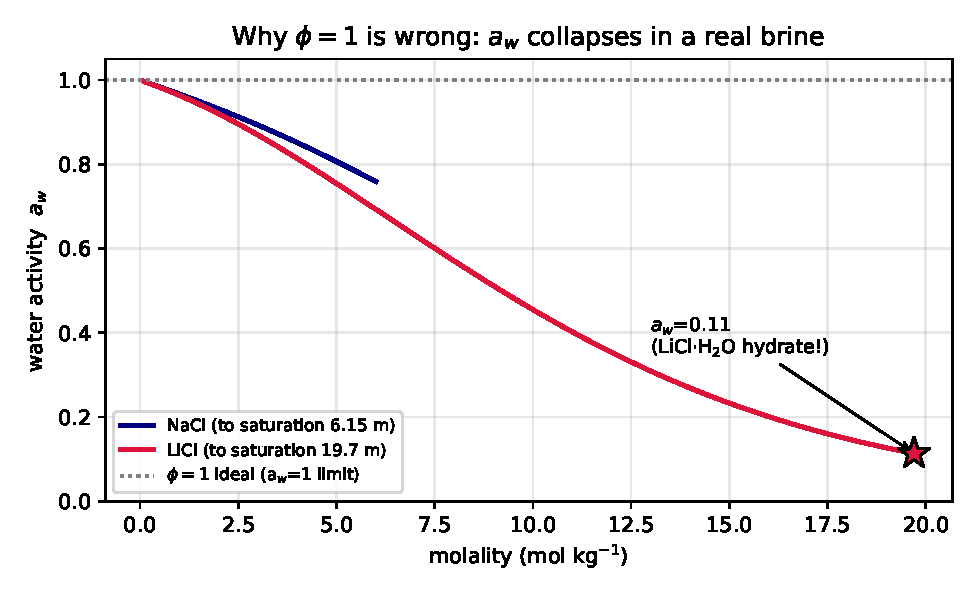
\includegraphics[width=\linewidth]{aw_collapse.pdf}
\end{columns}
\vspace{0.2em}
\footnotesize At LiCl saturation $a_w=0.11$ --- the hydrate equilibrium lives or
dies by it. (Implemented this in Choupo's \texttt{PitzerHMW}; the interface had
reserved the slot for it.)
\end{frame}

\begin{frame}{Validation of the water activity}
\begin{columns}
\column{0.5\textwidth}
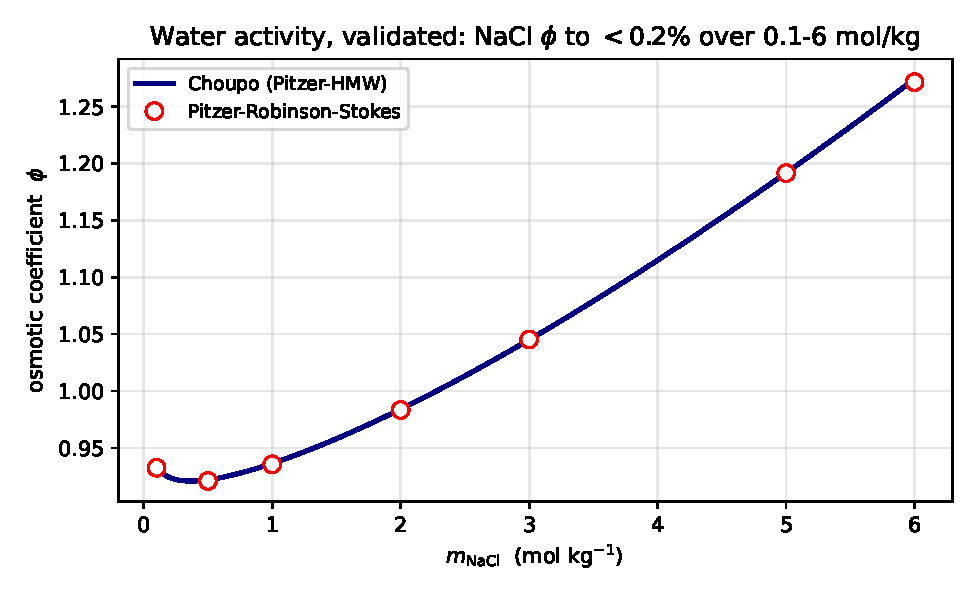
\includegraphics[width=\linewidth]{phi_nacl.pdf}
\column{0.5\textwidth}
\begin{itemize}
  \item NaCl $\phi$ vs Pitzer--Robinson--Stokes, $0.1$--$6$\,mol/kg: \textbf{$<0.2\%$}.
  \item Seawater $a_w = 0.981$ (measured $0.980$--$0.981$).
  \item Single-salt $\phi$ oracle to $10^{-15}$.
  \item \textbf{Independent adversarial audit} (four expert reviewers, term by
        term vs Pitzer 1991 / HMW 1984): zero defects.
\end{itemize}
\vspace{0.4em}
\begin{block}{}
\small This is what ``glass-box'' buys: the validation is \emph{in the repository},
reproducible, and was \emph{tried to be broken} on purpose.
\end{block}
\end{columns}
\end{frame}

% ===================== PART IV : PREDICTION =====================
\section{Prediction --- Farelo's NaCl + NH$_4$Cl}

\begin{frame}{The data: Prof.\ F\'atima Farelo (DEQ), JCED 2005}
\footnotesize Farelo, Fernandes \& Avelino, \emph{Solubilities for Six Ternary
Systems\ldots at $T=(298$--$333)$\,K}, J.\ Chem.\ Eng.\ Data \textbf{50} (2005)
1470. DOI 10.1021/je050111j.
\vspace{0.4em}
\begin{itemize}\small
  \item Six chloride ternaries; saturation molalities to $\pm0.0007$\,mol/kg.
  \item Pure-salt anchors (298\,K): NaCl 6.15, NH$_4$Cl 7.35, LiCl 19.7\,mol/kg.
  \item NaCl+NH$_4$Cl: simple eutonic, no double salt --- an \emph{experimental}
        fact the model assumes.
\end{itemize}
\begin{alertblock}{The test}
Calibrate the model to \emph{only} the two pure solubilities. Then \emph{predict}
the mixed-system saturation, and compare to her measured points.
\end{alertblock}
\end{frame}

\begin{frame}{What Farelo measured}
\textbf{The measured quantity:} the composition of the \emph{saturated solution} ---
the molality of \emph{each} salt in the liquid in equilibrium with the solid
phase(s) --- mapped from one pure-salt edge to the other, on isotherms at
$T=(298,\,313,\,333)$\,K (some series to 340\,K).
\vspace{0.3em}
\centering\scriptsize
\begin{tabular}{lcccl}
\toprule
ternary & $T$/K & \multicolumn{2}{c}{measured molality range (mol/kg)} & solid phase(s) \\
\midrule
NaCl+NH$_4$Cl & 298--333 & NaCl 3.9--6.15 & NH$_4$Cl 4.35--7.35 & NaCl + NH$_4$Cl \\
KCl+NH$_4$Cl  & 298--333 & KCl 2.23--2.43 & NH$_4$Cl 5.75--8.82 & KCl + NH$_4$Cl \\
NaCl+LiCl     & 298--333 & NaCl 0.03--6.15 & LiCl 19.7--23.5 & \textbf{LiCl$\cdot$H$_2$O} \\
KCl+LiCl      & 298--333 & KCl 0.87--4.78 & LiCl 19.7--23.5 & \textbf{LiCl$\cdot$H$_2$O} \\
NaCl+AlCl$_3$ & 298--338 & NaCl 0.17--6.15 & AlCl$_3$ 3.24--3.45 & \textbf{AlCl$_3\cdot$6H$_2$O} \\
KCl+AlCl$_3$  & 298--338 & KCl 0.57--4.78 & AlCl$_3$ 3.12--3.45 & \textbf{AlCl$_3\cdot$6H$_2$O} \\
\bottomrule
\end{tabular}
\vspace{0.4em}
\flushleft\footnotesize
\textbf{How:} visual polythermal (synthetic) method, sealed cell $\pm0.03$\,K
(chloride fields); isothermal equilibration $+$ AgNO$_3$ potentiometric Cl$^-$
titration ($\pm0.8\%$) $+$ AAS (Li/Al systems). Saturation molalities to
$\pm0.0007$\,mol/kg. \\
\textbf{And:} the \emph{solid phase itself} --- eutonic (no double salt) vs
hydrate vs hydrolysis --- an experimental finding the model cannot guess.
\end{frame}

\begin{frame}{All 553 measured points}
\centering
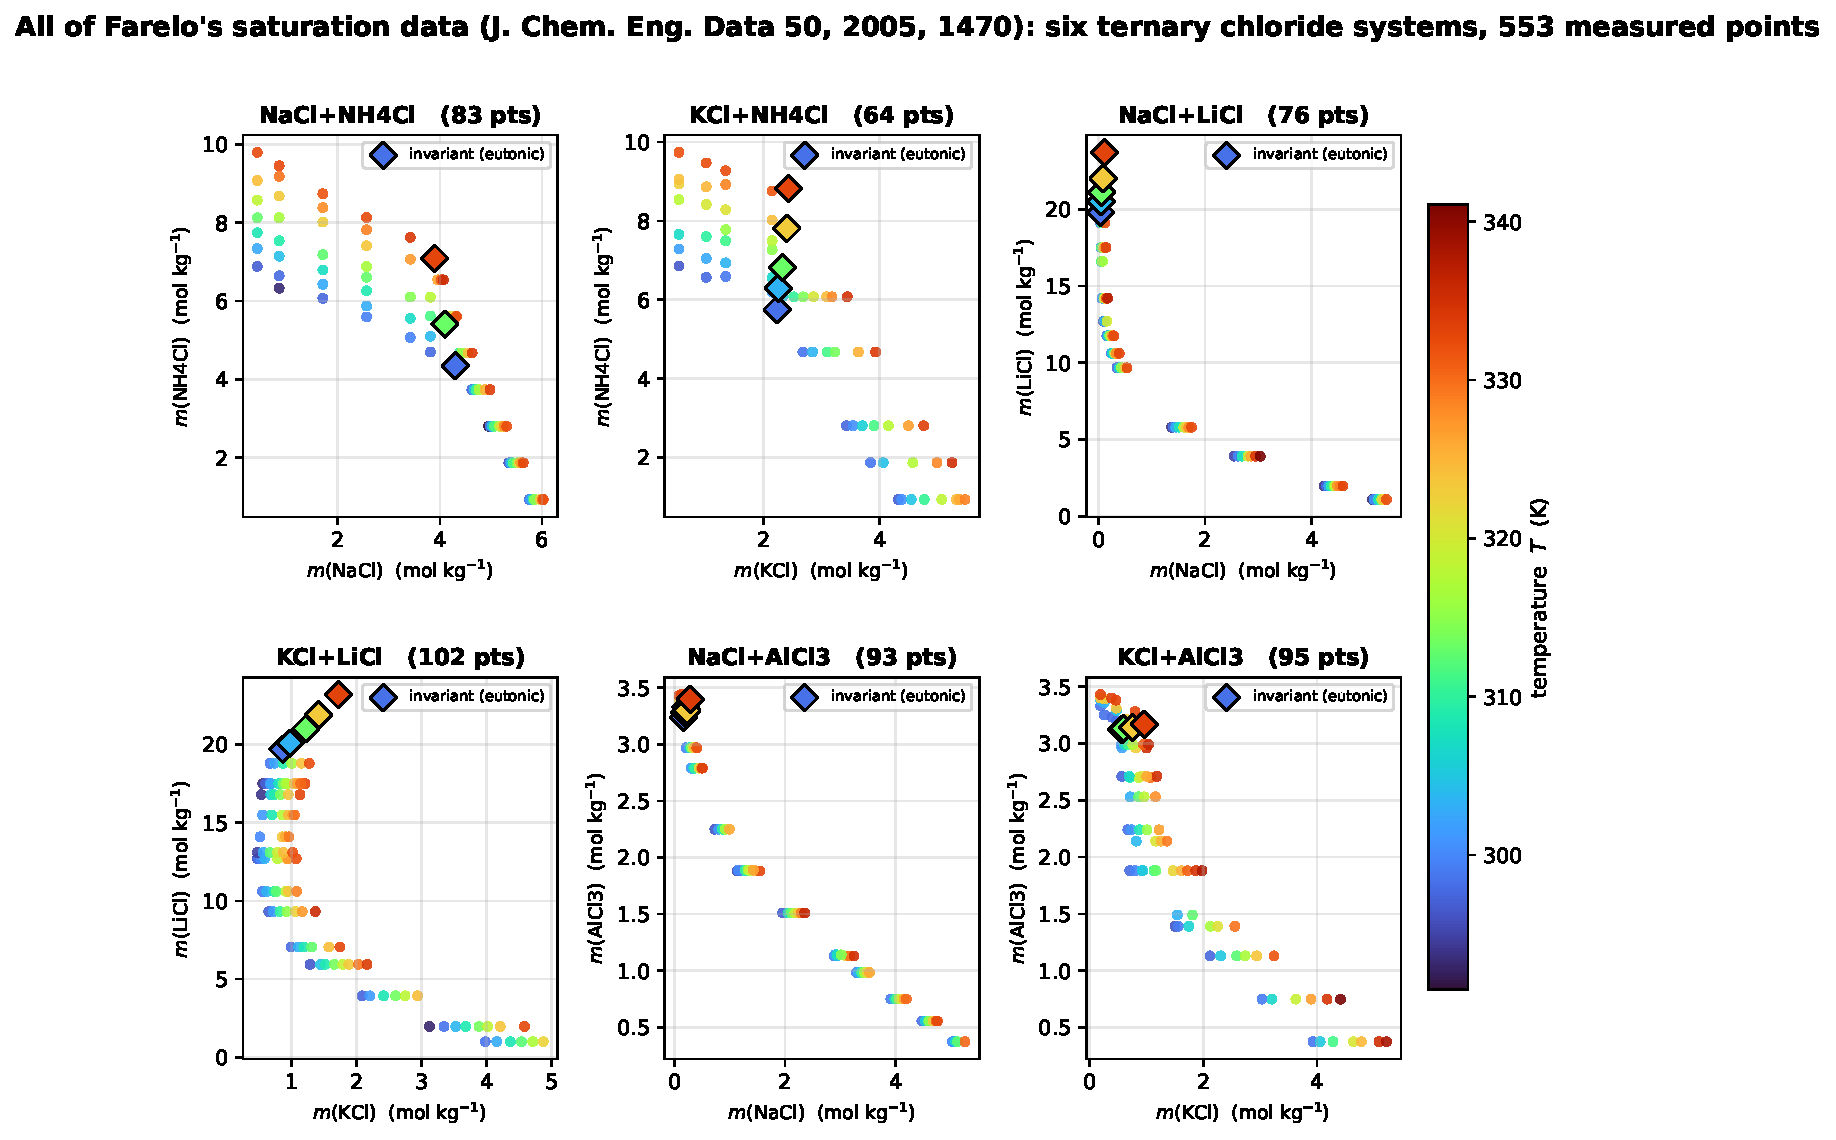
\includegraphics[height=0.82\textheight]{farelo_all.pdf}\\[-0.2em]
{\footnotesize Every saturated composition from the paper's twelve tables ---
six ternary systems, coloured by temperature. The full dataset now lives, cited,
in each case's \texttt{constant/experimental/farelo\_solubility.csv}.}
\end{frame}

\begin{frame}{The plan: predict, regress --- and \emph{where} it is stored}
\small One thermodynamic model throughout: \textbf{Pitzer--Harvie--M\o ller--Weare}
($\gamma_i$ + the osmotic $a_w$) for the liquid, $K_{sp}$ for each solid.
\vspace{0.3em}
\begin{center}
\begin{tabular}{llll}
\toprule
systems & what we do & parameters \emph{obtained} & saved in \\
\midrule
NaCl/KCl & \textbf{predict} the & NH$_4$--Cl $\beta^0,\beta^1,C^\phi$ & \texttt{pairs.dat} \\
\ + NH$_4$Cl & ternary; fit one $K_{sp}$ & sal-ammoniac $\log K_{sp}$ & \texttt{minerals.dat} \\[3pt]
NaCl/KCl & \textbf{regress} (refit) to & Li--Cl $\beta^0,\beta^1,C^\phi$ (refit) & \texttt{pairs.dat} \\
\ + LiCl & reach saturation & LiCl$\cdot$H$_2$O $\log K_{sp}$ & \texttt{minerals.dat} \\
 & & Li$^+$ $\Delta_f H^\circ_{\rm aq}$ & \texttt{ions.dat} \\[3pt]
NaCl/KCl & \textbf{defer} --- needs an & \emph{(none yet)} & --- \\
\ + AlCl$_3$ & Al$^{3+}$ hydrolysis model & & \\
\bottomrule
\end{tabular}
\end{center}
\vspace{0.3em}
\begin{block}{}
\small Every obtained parameter becomes a \emph{permanent, sourced} line in
\texttt{data/standards/electrolyte/} --- cited to Farelo, read by name by the
engine, pinned by a validation case. (The exact \texttt{pairs.dat} entry: later.)
\end{block}
\end{frame}

\begin{frame}{The salting-out, in the ternary diagram}
\centering
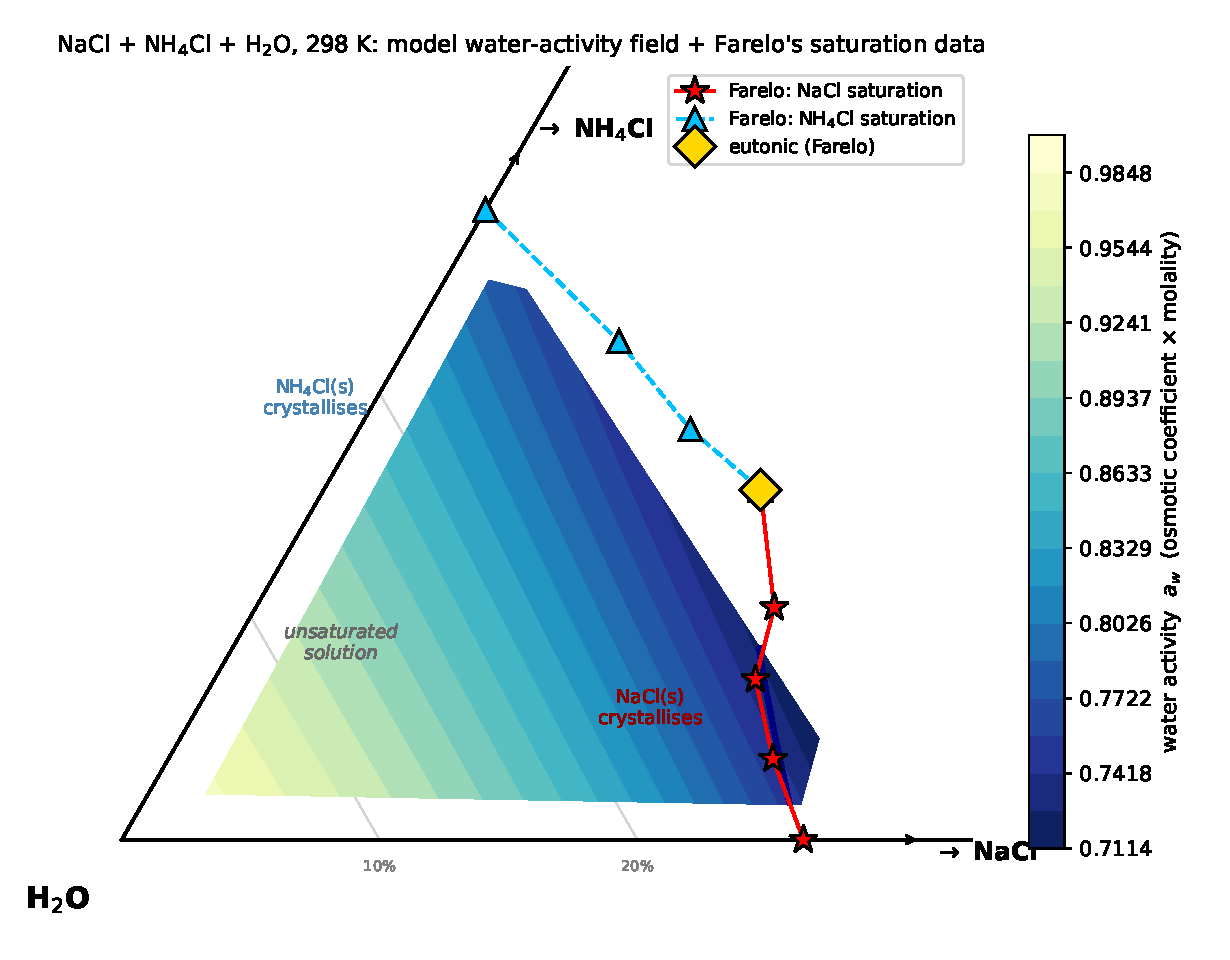
\includegraphics[height=0.80\textheight]{ternary_nacl_nh4cl.pdf}\\[-0.2em]
{\footnotesize The model's water-activity field (colour) with Farelo's two measured
saturation branches and the eutonic. $a_w$ falls $0.98\rightarrow 0.71$ toward
saturation --- the osmotic drive for crystallisation.}
\end{frame}

\begin{frame}{The common-ion salting-out, quantified}
\begin{columns}
\column{0.55\textwidth}
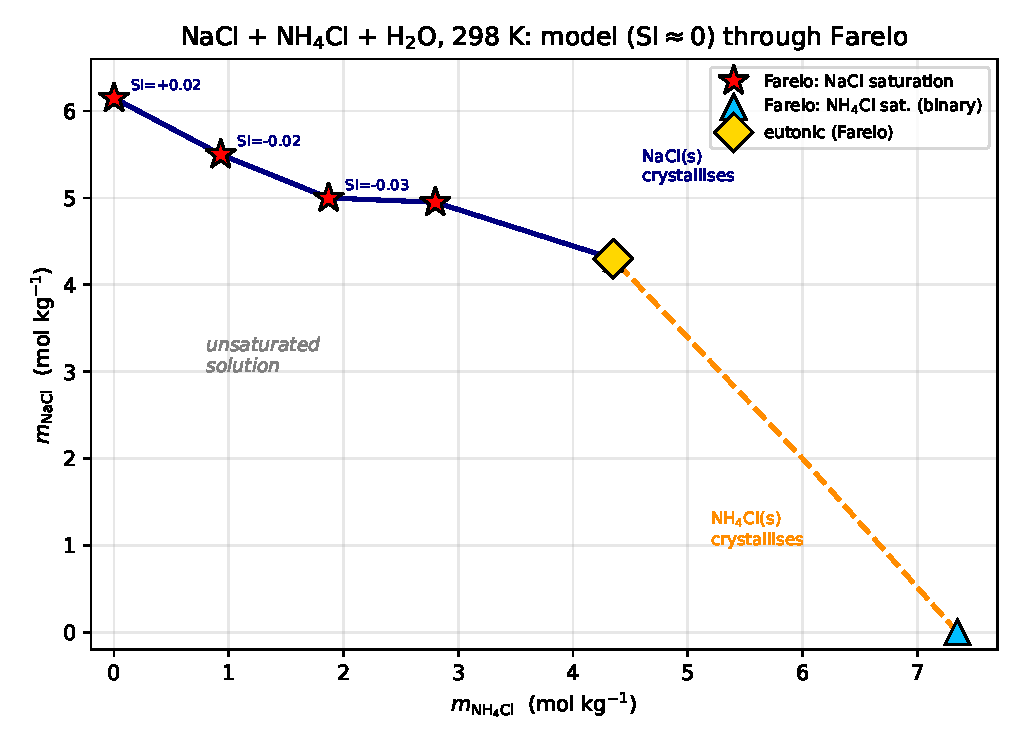
\includegraphics[width=\linewidth]{nacl_nh4cl_phase.pdf}
\column{0.45\textwidth}
\small
Adding NH$_4$Cl drives NaCl out of solution (shared Cl$^-$). The model's NaCl
saturation index at each of Farelo's \emph{measured} points:
\vspace{0.3em}
\begin{tabular}{lc}
\toprule
point & SI$_{\mathrm{halite}}$ \\
\midrule
NaCl 6.15 & $+0.017$ \\
+ NH$_4$Cl 0.93 & $-0.022$ \\
+ NH$_4$Cl 1.87 & $-0.028$ \\
NH$_4$Cl 7.35 & $-0.000$ \\
\bottomrule
\end{tabular}
\vspace{0.4em}
\textbf{$\pm0.03$ log units.} The IST simulator reproduces the IST measurements.
\end{columns}
\end{frame}

% ===================== PART V : RECALIBRATION =====================
\section{Recalibration --- Farelo's LiCl}

\begin{frame}{LiCl: where the model first \emph{fails} --- then is fixed}
\begin{columns}
\column{0.56\textwidth}
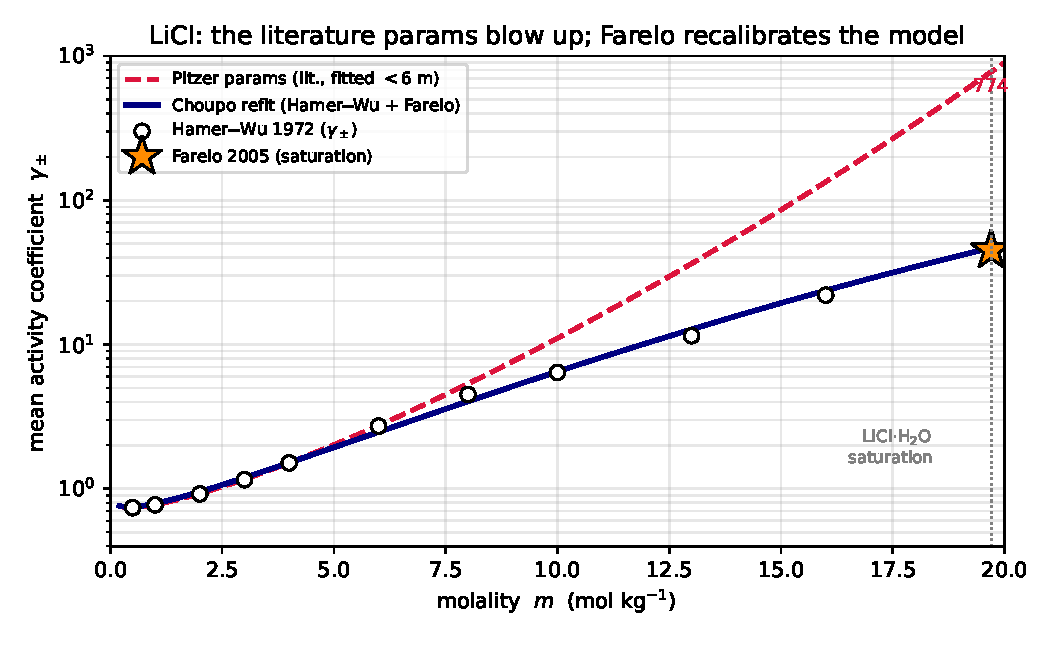
\includegraphics[width=\linewidth]{licl_gamma.pdf}
\column{0.44\textwidth}
\small
LiCl saturates at $\sim$20\,mol/kg. The literature parameters (fitted $<$6\,m)
give $\gamma_\pm=774$ vs $\sim$45 measured.
\vspace{0.4em}
\textbf{Don't declare defeat --- use the measurement.} Refit $\beta,C^\phi$ to
Hamer--Wu $\gamma_\pm$ \emph{and} Farelo's saturation. A \emph{negative} $C^\phi$
tames the blow-up; the model now tracks LiCl to $\sim$11\% \emph{to saturation}.
\vspace{0.4em}
And the LiCl$\cdot$H$_2$O hydrate $K_{sp}$ closes \emph{through} the osmotic
$a_w=0.11$ --- the two pieces of this talk meeting.
\end{columns}
\end{frame}

% ===================== PART VI : DATA FLOW =====================
\section{How a measurement enters the compound}

\begin{frame}{The data flow --- measurement $\rightarrow$ catalogue $\rightarrow$ engine}
\small
\begin{enumerate}
  \item \textbf{Measurement} (Farelo 2005): LiCl saturation 19.7\,mol/kg; NH$_4$Cl 7.35.
  \item \textbf{Curation} (a human act): fit / calibrate, with the \emph{primary}
        source cited per value. The engine \textbf{refuses} to write into
        \texttt{data/standards/} --- adding data is deliberate.
\end{enumerate}
\begin{exampleblock}{\footnotesize what actually lands in \texttt{electrolyte/pairs.dat}}
\tiny\ttfamily
\{ cation Li; anion Cl; beta0 0.17; beta1 0.278; Cphi -0.0026; \\
\ \ source "REFIT to Hamer \& Wu 1972 gamma\_pm + Farelo (JCED 50, 2005, 1470) \\
\ \ saturation, valid to \textasciitilde19 mol/kg; supersedes the Appelo 2014 low-m fit"; \}
\end{exampleblock}
\begin{enumerate}\setcounter{enumi}{2}\small
  \item \textbf{Engine} reads it \emph{by name}; \texttt{PitzerHMW} uses it; the
        run \emph{announces} the active parameters.
  \item \textbf{Validation case} pins the result to the measurement (a golden master).
\end{enumerate}
\centerline{\footnotesize The whole chain is open, sourced, and re-runnable --- the antithesis of the black box.}
\end{frame}

% ===================== PART VII : LESSON =====================
\section{The lesson}

\begin{frame}{Measurement and model --- each their part}
\begin{columns}
\column{0.5\textwidth}
\begin{block}{Where the model is valid}
it \emph{earns trust} by reproducing the measurement (NaCl+NH$_4$Cl, SI$\approx 0$).
The water activity becomes a \emph{prediction}, not a guess.
\end{block}
\column{0.5\textwidth}
\begin{block}{Where it fails}
the measurement is \emph{irreplaceable} (LiCl at saturation) --- and it
\emph{calibrates} the model so it can be extended \emph{honestly}.
\end{block}
\end{columns}
\vspace{0.8em}
\centering
A model that only reproduces what it was fitted to is \emph{consistent}; the
experiment that grounds it is what makes it \emph{useful}.\\[0.6em]
And in a glass box, the engineer can finally answer the old professor:\\[0.3em]
\textbf{\itshape ``Sim --- e eu posso ver, e perguntar, e pensar.''}
\end{frame}

\begin{frame}{Summary}
\begin{itemize}
  \item Simulators began \emph{open} and turned \emph{closed}; Choupo turns back
        --- glass-box, open, every equation visible and announced.
  \item A rigorous Pitzer--HMW electrolyte model and speciation solver, validated
        and \emph{adversarially audited}.
  \item Farelo's NaCl+NH$_4$Cl: \textbf{predicted} to $\pm0.03$ log units.
  \item Farelo's LiCl: \textbf{recalibrated} the standard parameters, and the
        hydrate closed through the osmotic water activity.
  \item A respected IST colleague's dataset is now the reference curve for an
        open, IST-built simulator.
\end{itemize}
\vspace{0.8em}
\centering\large Obrigado --- e obrigado, Professora Farelo.
\end{frame}

\end{document}
